% !TEX encoding = UTF-8
% !TEX TS-program = pdflatex
% !TEX root = ../tesi.tex

%**************************************************************
\chapter{Resoconto dello stage}
\label{cap:resoconto-stage}
%**************************************************************

\intro{In questo capitolo verranno descritte le attività svolte durante lo stage. Per ogni attività si cercherà di descrivere il problema affrontato, le scelte effettuate ed i test svolti.}\\

\section{Pianificazione}
La prima attività svolta, in realtà ancora prima dell'inizio dello stage stesso, è stata quella di pianificare il lavoro da svolgere. Tale pianificazione è stata concordata tra il tutor aziendale e il sottoscritto, ed è esposta nella sezione \ref{sec:vincoli-temporali} a pagina \pageref{sec:vincoli-temporali} di questo documento.\\
Tale pianificazione, però, è stata "aggiustata" (ma mai stravolta) in base a quanto svolto settimana per settimana, decidendo di dedicare più o meno ore ad una determinata attività.\\
Al termine di ogni settimana, periodo coincidente con il raggiungimento di un obiettivo, infine, è stato deciso che avrei dovuto redarre una breve relazione, con lo scopo di documentare il lavoro svolto. Tali relazioni, inoltre, sono servite come materiale ausiliario per la presentazione delle nuove funzionalità sviluppate al proponente. Infine, terminati tutti gli obiettivi e in caso di approvazione da parte del tutor e del proponente, avrei dovuto trasferire il lavoro svolto dall'ambiente di sviluppo a quello di produzione.

\section{Funzionamento e struttura del Booking Engine}
Appena iniziato lo stage, mi sono subito dedicato all'analisi della struttura di CrociereRegalo, grazie anche (soprattutto all'inizio) all'aiuto del mio tutor. 
\subsection{Funzionalità}
CrociereRegalo è un motore di ricerca di crociere. Permette di trovare una determinata crociera utilizzando dei filtri di ricerca per area geografica (ad esempio Caraibi, Mediterraneo, Nord Europa), per data di partenza con granularità mensile (ad esempio Settembre 2018), per intervalli di durata (da 1-6, 7-8, 9-12 o più di 12 giorni) e per compagnia di crociera (ad esempio MSC Crociere). Per capire bene il suo funzionamento è stato necessario apprendere alcuni termini tecnici affini all'ambiente croceristico, come :
\begin{itemize}
	\item \textbf{Itinerario}: definisce il percorso che fa una crociera (ad esempio "Barcellona, Ajaccio, Civitavecchia, Barcellona"). Nell'arco di un periodo di tempo vi possono essere molteplici crociere percorrenti un singolo itinerario. Ogni itinerario è identificato da un codice che lo contraddistingue univocamente, e la durata dell'itinerario è una proprietà intrinseca (ovvero, all'interno di una compagnia di crociera, non esistono due itinerari che svolgono lo stesso percorso mettendoci tempi diversi). Ciascun itinerario ha 0 o più partenze nell'arco di un anno;
	\item \textbf{Cabina}: é una stanza di una nave da crociera. Esistono varie categorie di cabina, differenziate in base alla grandezza, al posizionamento (ad esempio le cabine interne alla nave, senza quindi finestre, che sono quelle più economiche). Quando si effettua una prenotazione, non viene prenotato un posto letto ma viene prenotata un'intera cabina;
	\item \textbf{Opzione}: consiste nel blocco del prezzo di una cabina per un periodo di tempo che varia in base al fornitore, ma che di solito si attesta tra le 24 e le 72 ore. Tale prezzo infatti, analogamente per quanto avviene con i biglietti aerei, aumenta all'aumentare delle prenotazioni (quindi al passare del tempo).

\end{itemize}
Premesso ciò, CrociereRegalo permette di selezionare un itinerario, vederne le partenze, categorie di cabina disponibili e prezzi e poi prenotare od opzionare una cabina. 

\subsection{OTA e DataExchange}
Mi è stato spiegato che il Booking Engine, in realtà, era spezzato in due parti dipendenti l'una dall'altra: \textbf{OTA} (disponibile all'indirizzo \url{https://www.crociereregalo.it}) e \textbf{DataExchange} (disponibile all'indirizzo \url{https://data.crociereregalo.it}). L'idea alla base di questa divisione è che la parte \textit{OTA} rappresenti il sito web vero e proprio, con il quale l'internauta si affaccia, mentre la parte \textit{DataExchange} serva per l'interazione tra \textit{OTA} e \glspl{webservice} dei vari fornitori (dove per fornitori si intendono le varie compagnie di crociera). 

\subsection{Interazione tra OTA e DataExchange}
\textit{OTA} e \textit{DataExchange} sono sì dipendenti l'uno dall'altro, ma hanno due database separati. Questo, fondamentalmente, avviene perchè i dati provenienti da i vari fornitori hanno formati diversi, che devono quindi essere uniformati per poter essere processati secondo una logica più indipendente possibile. Il compito del \textit{DataExchange} è proprio questo: interrogare i \glspl{webservice} dei vari fornitori, ricevere i dati, elaborarli, uniformarli e passarli ad \textit{OTA}.\\
Premesso ciò, vi sono due possibili interazioni tra \textit{OTA} e \textit{DataExchange}
\begin{itemize}
	\item Interazione \textbf{schedulata}, che avviene circa 3 volte al giorno, il cui compito è sincronizzare i cataloghi (chiamati anche \textit{flatfile}) dei vari fornitori per rendere disponibili le (eventuali) modifiche alla parte \textit{OTA} del Booking Engine. \\Quando un visitatore del sito CrociereRegalo cerca una crociera, tale ricerca avviene interrogando i cataloghi presenti nel database della parte \textit{OTA}, senza quindi interrogare i \glspl{webservice} delle compagnie di crociera (per motivi di prestazione dovuti all'ingente mole di dati da elaborare). I cataloghi, quindi, vengono scaricati nel DataExchange, elaborati (uniformati) e poi sincronizzati con il database di OTA; la procedura di sincronizzazione viene chiamata \textbf{Integrazione}. L'integrazione avviene attraverso l'invocazione (grazie allo scheduler di \textit{Windows Server}) che, grazie ad una chiamata \textit{HTTP} ad una particolare pagina del DataExchange, invoca la procedura di integrazione dati.
	\begin{figure}[!h] 
		\centering 
		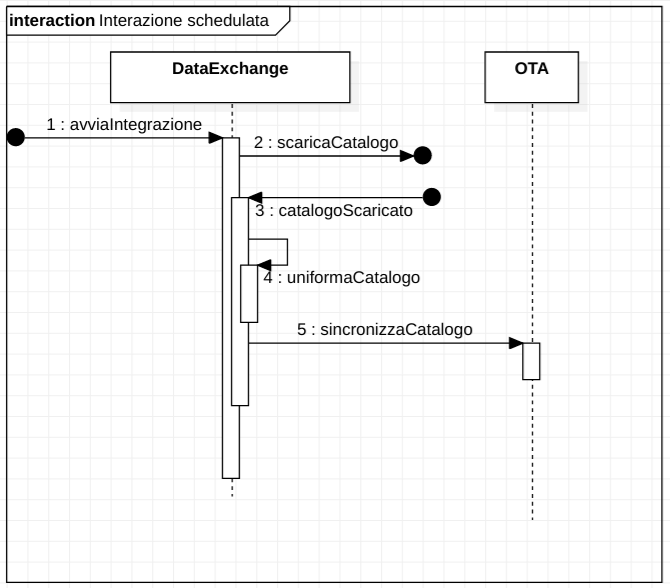
\includegraphics[width=.75\columnwidth]{attivita/interazione_schedulata} 
		\caption{Schema dell'integrazione schedulata appena descritta.}
	\end{figure}
	\item Interazione \textbf{real-time}, che avviene durante tutto il flusso di prenotazione di una cabina (che analizzerò in seguito). Tale flusso deve per forza disporre di dati aggiornati in tempo reale, altrimenti potrebbero verificarsi problemi in fase di prenotazione (come la prenotazione di una cabina non più disponibile). L'interazione in tempo reale avviene attraverso delle chiamate \textit{HTTP} (ajax) effettuate nel momento del bisogno dall'\textit{OTA} al \textit{DataExchange}, attraverso lo scambio di dati in formato \textit{JSON}.
	\begin{figure}[!h] 
		\centering 
		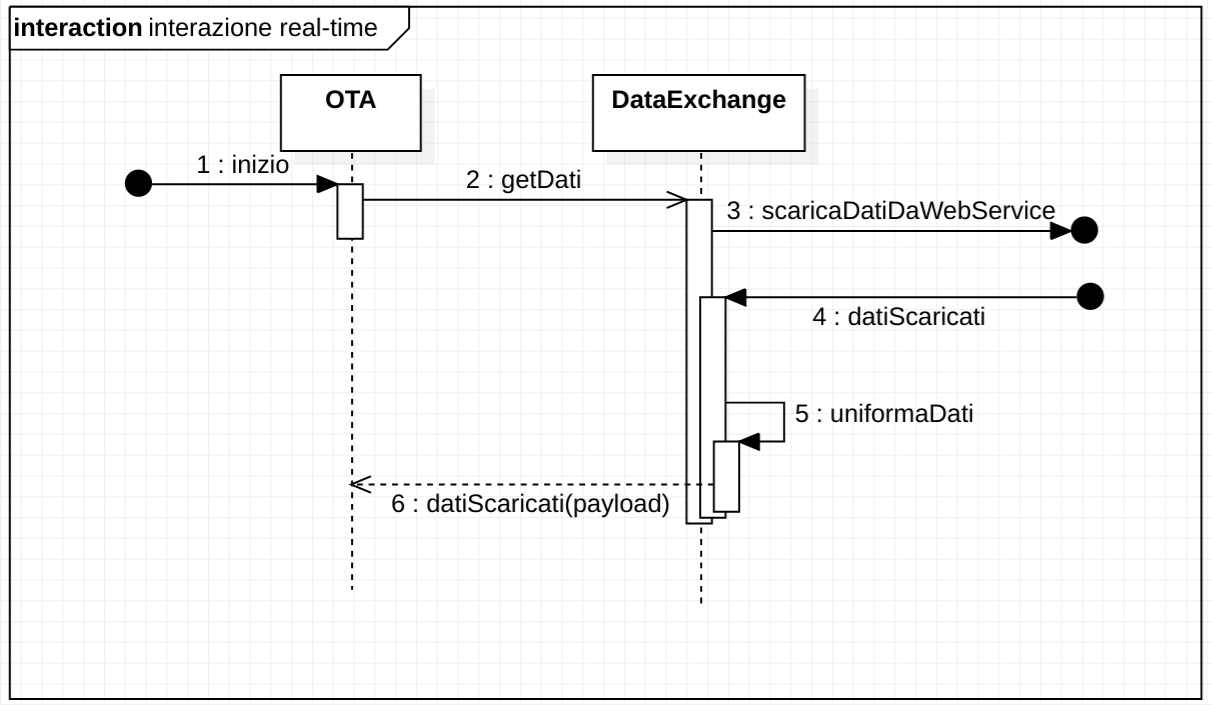
\includegraphics[width=.75\columnwidth]{attivita/interazione_realtime} 
		\caption{Schema dell'integrazione in tempo reale appena descritta.}
	\end{figure}
\end{itemize}

\subsection{Flusso di prenotazione}
Quando il visitatore, in seguito alla ricerca, apre i dettagli di una partenza, viene data la possibilità di poter avviare la procedura (flusso) di prenotazione, che si avvale dell'interazione real-time tra \textit{OTA} e \textit{DataExchange} si compone nei seguenti punti:
\begin{enumerate}
	\item \textit{categoryAvailability}: vengono elencati i gruppi (categorie) di cabine effettivamente disponibili (o un messaggio di errore in caso non vi siano più posti prenotabili) tenendo conto del numero di passeggeri inseriti (banalmente, se si selezionano 4 passeggeri, vengono mostrati le categorie di cabine nelle quali vi è presente almeno una quadrupla) e dell'età di tali passeggeri (per il calcolo preciso della tariffa, in quanto un minore paga meno di un adulto);
	\item \textit{cabinAvailability}: una volta selezionato una categoria di cabine, vengono mostrate tutte le cabine (una per una) ancora disponibili, raggruppate in base al ponte della nave in cui si trovano;
	\item \textit{categoryItem}: vengono elencati tutti i servizi extra (e relativi prezzi) disponibili in aggiunta a quelli già inclusi nel prezzo della cabina, e viene data la possibilità di selezionarli per aggiungerli alla prenotazione;
	\item \textit{requestPricing}: viene mostrato il prezzo finale (preso dal \gls{webservice} del fornitore) della prenotazione, tenendo conto di quanto selezionato negli step precedenti. Tale prezzo include anche le tasse portuali ed eventuali oneri aggiuntivi;
	\item \textit{requestBooking}: viene effettuata una prenotazione od un'opzione di quanto selezionato negli step del flusso precedenti. Nel caso di prenotazione, viene anche gestito il pagamento (tramite \gls{api} fornite dal consorzio \textit{Triveneto Bassilichi}).
\end{enumerate}

\subsection{Struttura del codice}
Sia \textit{OTA} che \textit{DataExchange} sono realizzati usando il framework \textit{Codeigniter}. Questo implica che applicano a PHP il paradigma \textit{Object-oriented} (orientato agli oggetti) associato al design pattern \gls{mvc}. Entrambi i progetti, dunque, presentano tre tipologie di classi:
\begin{itemize}
	\item \textbf{Model}, che estendono la classe base \textit{CI\_Model}, i quali sono la chiave di accesso ai dati dell'applicazione. Si è deciso di realizzare un \textit{model} per ogni tabella presente nel database;
	\item \textbf{View}, che generano il codice HTML di ogni pagina (o porzione di essa). Alle \textit{view} é possibile passare delle variabili in modo da rendere dinamico il loro contenuto.
	\item \textbf{Controller}, che estendono la classe base \textit{CI\_Controller} e istanziano le \textit{view} popolandole con i dati provenienti dai \textit{model}. La particolarità di queste classi è che i loro metodi pubblici si possono chiamare direttamente tramite URL. Codeigniter, infatti, implementa un meccanismo (grazie al \textit{magic method \_\_call}) per il quale é possibile chiamare un metodo pubblico \textit{a} di una classe controller \textit{C} semplicemente recandosi all'url \textit{nomedelsito.dominio/C/a} (ad esempio \textit{crociereregalo.it/C/a}). Tale meccanismo risulta molto utile nella realizzazione di \gls{api} e nella creazione di \textit{URL} user-friendly (quindi più leggibili)
\end{itemize} 
Codeigniter, inoltre, presenta un modulo personalizzato per interagire con il database, che supporta funzionalità come il \textit{log delle query} (in pratica è possibile sapere l'ultima query eseguita, molto utile in caso di debug), meccanismi di \textit{query builder} (creazione assitita di query), \textit{query parametrizzate}, gestione delle transazioni ecc.
